\documentclass[12pt,oneside,a4paper]{article}   
\usepackage[czech, english]{babel}
\usepackage{amsmath}
\usepackage{epsf,epic,eepic,eepicemu,url}
\usepackage[utf8]{inputenc}
\usepackage{graphicx}
\usepackage{algorithm2e}
\usepackage[section,subsection,subsubsection]{extraplaceins}
\newenvironment{listing}
{\begin{list}{}{\setlength{\leftmargin}{1em}}\item\scriptsize\bfseries}
{\end{list}}

\begin{document}
\begin{center}
\bf Semestralní projekt MI-PAA 2012/2013:\\[5mm]
     Řešení problému vážené splnitelnosti booleovské formule pokročilou iterativní metodou\\[5mm]
       Jiří Špaček (spaceji3@fit.cvut.cz)\\[2mm]
magisterské studium, FIT ČVUT\\[2mm]
\end{center}

\section{Zadání práce}

Cílem práce je navrhnout a implementovat algoritmus pokročilé lokální heuristiky pro řešení problému vážené  splnitelnosti booleovské formule. Dalším úkolem práce bylo provedení experimentálního ověření výkonnosti implementovaného algoritmu a na základě naměřených výsledků navrhnout optimální hodnoty parametrů algoritmu.

\section{Definice problému}

Je dána booleovská formule $F$ proměnných $X=(x_1, x_2, … , x_n)$ v konjunktivní normální formě (tj. součin součtů). Dále jsou dány celočíselné kladné váhy $W=(w_1, w_2, … , w_n)$. Najděte ohodnocení $Y=(y_1, y_2, … , y_n)$ proměnných $x_1, x_2, … , x_n$ tak, aby $F(Y)=1$ a součet vah proměnných, které jsou ohodnoceny jedničkou, byl maximální. 

\section{Popis implementovaného algoritmu}

Pro implementaci algoritmu byla zvolena iterativní heuristika v podobě evolučního algoritmu. Tento algoritmus reflektuje proces proces přirozeného evolučního výběru známého z biologie.

Základní princip funkce evolučního algoritmu spočívá v iterativním zlepšování zdatnosti populace jedinců, reprezentovaných svojí genetickou informací (chromozómem).


Základní běh evolučního algoritmu je možné sledovat na následujícím pseudokódu:

\begin{listing}
\begin{verbatim}

function GeneticHeuristic(instance, stoppingCriterionFn, scalingSchemeFn, 
                           selectionFn, crossoverFn. mutationFn) {
 
  population = InitRandomPopulation(instance)
 
  while (not stoppingCriterionFn(population)) {
    // preskalovani genomu tvoricich populaci
    oldPopulation = Rescale(population, scalingSchemeFn)
    newPopulation = Breed(oldPopulation, selectionFn, crossoverFn, mutationFn)
    population = Repopulate(oldPopulation, newPopulation)
  }
}
 
 
function Breed(population, selectionFn, crossoverFn, mutationFn) {
  newPopulation = Nil
  for i from 0 to Size(population) / 2 {
    genome1 = selectionFn(population)
    genome2 = selectionFn(population)
    offspring[] = crossoverFn(genome1, genome2)
    mutationFn(offspring[0])
    mutationFn(offspring[1])
    newPopulation->Add(offspring)
  }
  return newPopulation
}


\end{verbatim}
\end{listing}

Algoritmus začíná vygenerovaným náhodné populace jedinců. Následuje cyklické opakování jednotlivých bloků algoritmu dokud není dosaženo ukončovací podmínky (implementována jako limit počtu iterací cyklu). Samotná iterace probíhá v následující posloupnosti kroků:
\begin{enumerate}
\item přeškálování zdatnosti - v tomto kroku dojde k přepočítání hodnot zdatnosti chromozomů z populace $P(t-1)$ za použití škálovací funkce.
\item selekce - výběr jedinců z původní populace dle výběrového mechanizmu zohledňujícího zdatnost těchto jedinců
\item křížení - aplikace binárního operátoru $S \times S \rightarrow S \times S$ kde $S$ je množina chromozomů. Účelem operátoru křížení je zajištění vzniku nové genetické informace ze dvou potenciálně vhodných rodičů.
\item mutace - aplikace unárního operátoru $S \rightarrow S$, která zajistí 
\item re-populace - Vytvoření nové populace $P(t)$ na základě výběrového mechanizmu upřednostňujícím ty nejzdatnější jedince vzniklých během operace křížení (popř. mutace), s použitím případného elitismu (tj. zachování několika nejlepších jedinců z populace $P(t-1)$)
\end{enumerate}

\subsection{Volba implementace funkčních bloků algoritmu}

Jednotlivé bloky navrženého algoritmu jsou plně konfigurovatelné a rozšiřitelné. Popis jednotlivých bloků a podporované konfigurace jsou shrnuty v následujícím seznamu:

\subsubsection{Selekce}
Za účelem výběru jedinců určených pro aplikaci operace křížení byl zvolen mechanizmus ruletového výběru, který

\subsubsection{Křížení}

Kontrola aplikace operátoru křížení je možné nastavit hodnotou $p_c$ udávající pravděpodobnost s jakou bude operace provedena. Celkem byly implementovány 3 druhy operátorů křížení:
  \begin{itemize}
    \item jednobodové křížení
    \item dvoubodové křížení
    \item uniformní křížení
  \end{itemize}
\subsubsection{Mutace} Operátor mutace je implementován jako operace negace bitu chromozómu, který je proveden v případě, že náhodný hod převýší stanovenou pravděpodobnost $p_m$.

\subsubsection{Repopulace} 
V rámci tohoto bloku je provedeno nahrazení všech konfigurací z generace $P(t-1)$ instancemi, které vznikly jako výsledek práce algoritmu v aktuální iteraci. Bylo však žádoucí, aby tento blok zachovával následující dvě vlastnosti: 
  \begin{itemize}
    \item zabránění ztráty nejlepších jedinců z předchozí populace. Tohoto je docíleno aplikací elitismu, kdy v z každé populace přecházejí do té nové 3 nejzdatnější jedinci.
    \item zabránění ztráty nalezeného (i když třeba nedokonalého) řešení - tj. takové instance, která splňuje vstupní formuli. Tímto je zvýšena šance, že algoritmus bude vracet použitelná řešení.
  \end{itemize}
  
\subsubsection{Škálovací funkce} Protože byla selekce navržena jako metoda ruletového výběru, bylo rozhodnuto o přidání funkce řízení selekčního tlaku na základě lineárního přeškálování instancí.

Celkem byly implementovány dva druhy přeškálování:

\subsubsection{Metoda lineárního škálování 1}

Založeno na zúžení nebo rozšíření oboru hodnot, ve kterém se pohybují hodnoty zdatností instancí populace $P(t-1)$. Zúžení oboru hodnot znamená snížení selekčního tlaku (pst. výběru nejlepšího jedince) a tedy zajišťuje nadržování slabším instancím a zvýší tím divergenci algoritmu. Rozšíření oboru hodnot naopak vede ke zvýšení selekčního tlaku.

Přepočet zdatností je proveden na základě funkce:

$f(z) = z_1 + (z - z_{min}) \frac{z_2 - z_1}{z_{max} - z_{min}}$

kde:
\begin{itemize}
\item $f(z)$ - je výsledná přeškálovaná zdatnost
\item $z$ - je původní zdatnost instance
\item $z_{max}$ - je zdatnost nejlepšího jedince
\item $z_{min}$ - je zdatnost nejhoršího jedince
\item $z_1$ - uživatelem definované nové minimum (zdatnost nejhoršího jedince)
\item $z_2$ - uživatelem definované nové maximum (zdatnost nejlepšího jedince)
\end{itemize}
Aby mohly být proměnné $z_1$ a $z_2$ nastavovány systematicky a to bez nutnosti znát skutečné hodnoty, se kterými alg. pracuje, rozhodl jsem se jejich volbu založily na jediném parametru $c_s$ (tzv. škálovacím koeficientu) definovaném v intervalu $(-1, 1)$, tak, aby volba mezních hodnot tohoto koeficientu zajišťovala následující vlastnosti:
\begin{itemize}
\item $c_s = -1$ - rozšíření oboru hodnot na dvojnásobnou šířku, což vede ke zvýšení selekčního tlaku.
\item $c_s = 0$ - přeškálování hodnoty zdatnosti nemění (funkce se chová jako identita)
\item $c_s = 1$ - přeškálování sjednotí všechny hodnoty zdatnosti na hodnotu $z_{max}$, čímž je zajištěn minimální selekční tlak.
\end{itemize}

Výpočet proměnných $z_1$ a $z_2$ je definován dle následujících vztahů:
\begin{itemize}
\item $z_1 =  z_{min} + (z_{max} - z_{min}) * c_s$
\item $z_2 = z_{max}$
\end{itemize}

Jakým způsobem jsou ovlivněny původní hodnoty je možné sledovat na následujícím grafu.

\begin{figure}[ht]
\centering
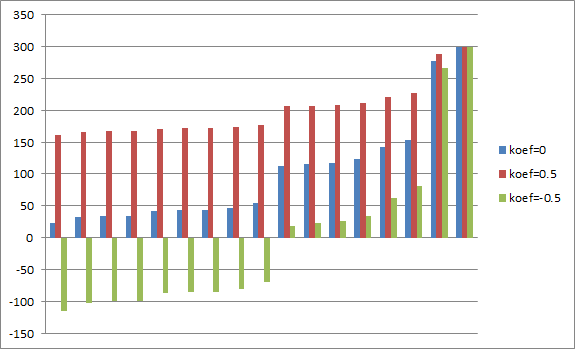
\includegraphics[scale=0.9]{obr/lin-scaling.png}
\caption{Ukázka lineárního přeškálování hodnot pro různé škálovací koeficienty}
\label{fig:figure1}
\end{figure}


\subsubsection{Metoda lineárního škálování 2}

Jako alternativa k předchozí metodě byla vybrána metoda navrhována v článku \uv{Scaling in Genetic Algorithms}. Přepočet zdatnosti je zde vyřešen na základě vztahu:
$f(z) = az + b$

Dále pak musejí být zachován určitý vztah mezi maximální zdatností nejlepšího jedince a průměrnou zdatností celé populace. Konkrétně se jedná o vztahy:
\begin{itemize}
\item $f'_{max} = f_{avg}c_s$
\item $f'_{avg} = f_{avg}$
\end{itemize}

Koeficient $c_s$ pak dovoluje řízení selekčního tlaku, kde jeho zvýšení vede ke zvýšení selekčního tlaku a naopak.

\subsubsection{Penalizační funkce}

Aby mohly být znevýhodněny instance, které porušují omezující podmínky problému (konfigurace porušuje omezující podmínky pokud nesplňuje některé klauzule) a docházelo tak přirozeně k jejich znevýhodnění při selekci, byla implementována penalizační funkce. Tato funkce zajistí zhoršení hodnoty zdatnosti. V rámci této práce bylo experimentováno se dvěma druhy penalizací:

První metoda spočívala na multiplikativní penalizaci, která zapříčiní zhoršení fitness hodnoty dle vztahu:

$f(z) = f_{raw}(z)p(z)$

Funkce $p$ byla definována jako poměr splněných klauzulí ku celkovému počtu klauzulí instance.

Druhá metoda spočívala v aditivní penalizaci definované dle vztahu:
$f(z) = f_{raw}(z) + c_pp(z)$

Penalizační funkce $p$ je definována jako:

$p(z) = \sum\limits_{c \in C_n}^{C_{n}} w_{max}(c)$

kde $C_n$ je množina nesplněných klauzulí instance $z$ a $w_{max}(c)$ je funkce, která vrátí největší váhu literálu, který je součástí klauzule $c$.

Koeficient $c_p$ pak slouží k správnému nastavení váhy penalizace.


\section{Experimentální ověření vlastností heuristiky}

\subsection{Měřené veličiny}

Aby bylo možné určit, které veličiny pro měření úspěšnosti algoritmu důležité, bylo nutné si nejdříve zodpovědět otázku, jak je vlastně kvalitní řešení definováno. V této práci je kvalita řešení posuzována podle dvou faktorů. 

Prvním je relativní chyba měření definovaná jako $\varepsilon = \frac{|C(OPT)-C(APX)|}{C(OPT)}$, kde $C(OPT)$ je hodnota fitness funkce optimálního řešení (zde zjištěného brute-force algoritmem) a $C(APX)$ je hodnota fitness funkce řešení vráceného heuristikou.

Druhým faktorem je hodnota poměru splněných instancí, ke všem řešeným instancím (jedná se o instance, které splňují omezující podmínky, ale nemusí být optimální).

Většina z měřených veličin je pak v rámci experimentů posuzována i vzhledem k obtížnosti instance z důvodu identifikace závislosti měřené veličiny na obtížnosti, s tím jak je měněn daný parametr algoritmu. Obtížnost instance $k$ je definována jako poměr počtu klauzulí ku počtu proměnných formule.

Z výsledků publikovaných v \uv{Stochastic Search And Phase Transitions:AI Meets Physics}(Selman) vyplývá, že největší obtížnosti dosahuji SAT instance, jejichž poměr $k$ je roven přibližně hodnotě 4,3.


\subsection{Výběr instancí problému}

Za účelem provedení experimentů byly použity instance knihovny SATLIB ve formátu DIMACS. Některé instance byly patřičně zkráceny, aby bylo dosaženo požadovaného poměru klauzulí k počtu proměnných. Protože SATLIB obsahuje instance s maximálním poměrem 91/20, byly za účelem testování algoritmu na instancích s $k>4,5$ tyto instance dogenerovány.

Celkem pak bylo prováděno testování na 6ti sadách s $k$ z množiny $\{1,2,3,4,5,6\}$, každá sada po 40ti instancích. Všechny instance byly splnitelné a bylo pro ně známo optimální řešení.


\subsection{Návrh experimentu}

V první fázi experimentu bylo provedeno několik základních experimentů, tak, aby mohlo být odhadnuto alespoň orientační nastavení počátečních parametrů algoritmu. Za tímto účelem bylo vybráno několik pokusných instancí s 40ti klauzulemi a 20ti proměnnými, nad kterými byla opakovaně spouštěna heuristika s různým nastavením parametrů.

Výsledkem bylo počáteční nastavení parametrů heuristiky, které v mnoha bodech vychází z výchozích hodnot:
\begin{itemize}
\item Velikost populace - 100
\item Počet generací - 300
\item Pravděpodobnost křížení - 100\%
\item Pravděpodobnost mutace - 10\%
\item Ruletový výběr, bez změny selekčního tlaku
\end{itemize}

V druhé fázi experimentu došlo k nastavení základních parametrů heuristiky počtu generací a velikosti populace. Optimální hodnoty těchto parametrů zjištěné v této fázi pak byly používány ve všech ostatních experimentech.

V další fází byl měřen vliv operátorů křížení a mutace na kvalitu výsledného řešení.

Na závěr byly otestovány dopady volby metod řízení selekčního tlaku a nastavení penalizací na kvalitu řešení.


\subsection{Měření vlivu počtu generací na kvalitu řešení}

Z výsledků prvního experimentu zaměřeného na sledování vývoje kvality řešení v závislosti na počtu iterací algoritmu je patrný vliv postupného zlepšování kvality řešení nejlepších jedinců, ze kterých se populace skládá.

\begin{figure}[ht]
\centering
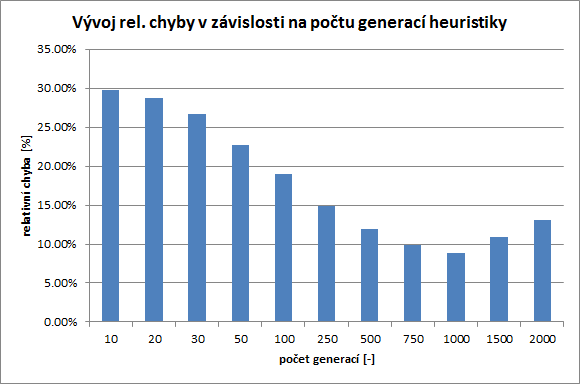
\includegraphics[scale=0.9]{obr/gen.png}
\end{figure}

\newpage
\FloatBarrier

\subsection{Měření vlivu velikosti populace na kvalitu řešení}

S růstem velikosti populace se dá předpokládat, že poroste i rozmanitost jedinců a tím pádem by měla stoupat i šance na nalezení potenciálně i těch zdatnějších než je tomu u populací menších.

Z výsledků experimentu je možné pozorovat, že instance nižších obtížností řeší heuristika i ve svém výchozím nastavení relativně úspěšně, z instancí s $k>=4$ je splnitelnosti dosaženo jen u necelé poloviny instancí, čehož je navíc dosaženo až při vyšších velikostech populace.

Tento trend se bohužel projevoval i u dalších experimentů a schopnost vyřešit i ty nejobtížnější instance se tak stal jedním z cílů, kterých mělo v rámci tohoto experimentu být dosaženo. 

Navíc protože tyto obtížné instance narušují výsledky dalších experimentů (mají vždy stejnou velikou chybu, kterou), přestávají v nich být patrné závislosti na nastavovaných parametrech, jsou následující experimenty omezeny pouze na lehčí instance.

Dalším důležitým pozorovatelným jevem je naplnění očekávaného chování heuristiky, kdy se zvyšujícím počtem jedinců dochází ke snížení rel. chyby. Jako optimální hodnota zde byla vybrána hodnota 100 jedinců populace.

\begin{figure}[ht]
\centering
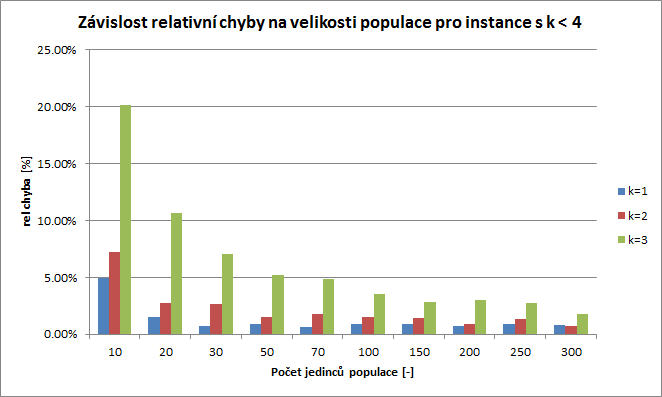
\includegraphics[scale=0.75]{obr/pop-size-err-min.png}
\end{figure}


\begin{figure}[ht]
\centering
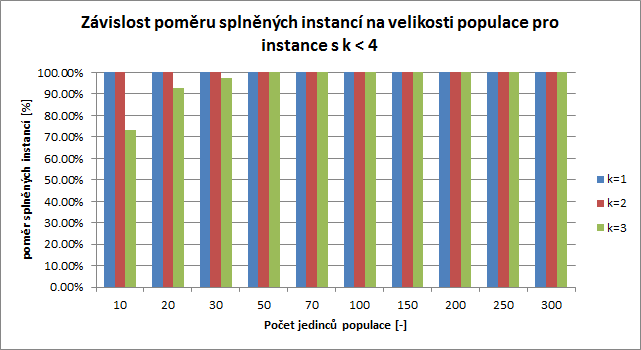
\includegraphics[scale=0.75]{obr/pop-size-sat-min.png}
\end{figure}

\begin{figure}[ht]
\centering
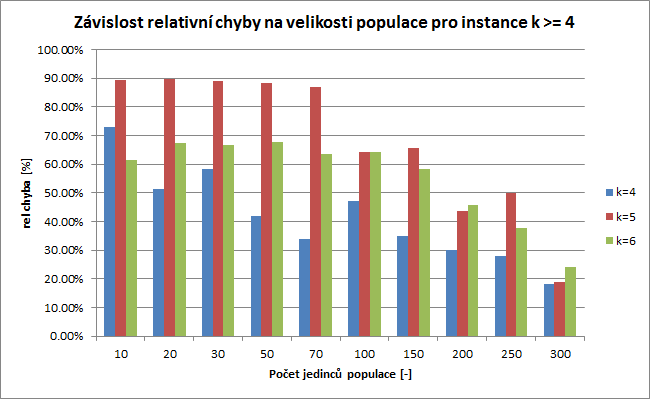
\includegraphics[scale=0.75]{obr/pop-size-err-max.png}
\end{figure}

\begin{figure}[ht]
\centering
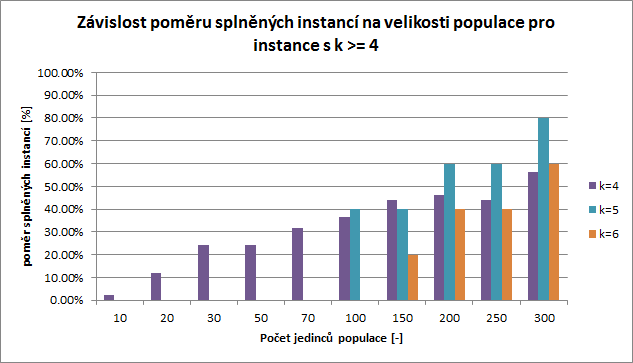
\includegraphics[scale=0.75]{obr/pop-size-sat-max.png}
\end{figure}

\newpage
\FloatBarrier

\subsection{Meření závislostí pravděpodobnosti mutace}

Úlohou operátoru mutace je vnesení náhodného šumu do instancí tvořících populaci a tím zajištění diverziti jedinců a zabránění degeneraci celé populace. Je však také možné očekávat, že s rostoucí hodnotou pravděpodobnosti mutace, bude vliv mutace převažovat nad selekčním tlakem a může tím dojít k divergenci celé populace s zhoršení výsledků heuristiky.

To se potvrzuje i na výsledcích dosažených v rámci experimentu, kdy pro vysoké hodnoty pst. mutace (>20\%) dochází k významnému zhoršení relativní chyby výsledných řešení.

Jako optimální nastavení pravděpodobnosti mutace jednoho bitu se jeví její nastavení někde v intervalu $1\% < x < 5\%$.

\begin{figure}[ht]
\centering
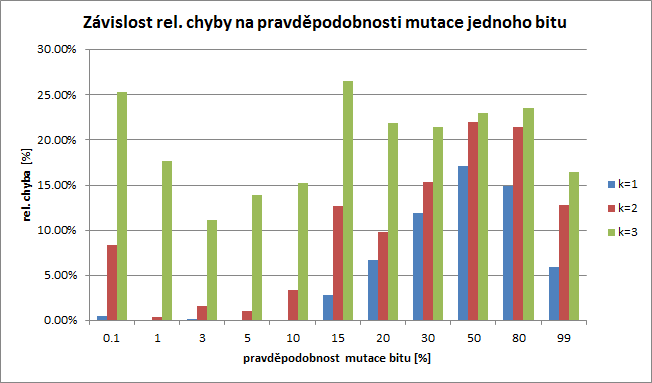
\includegraphics[scale=0.9]{obr/mut-err.png}
\end{figure}


\begin{figure}[ht]
\centering
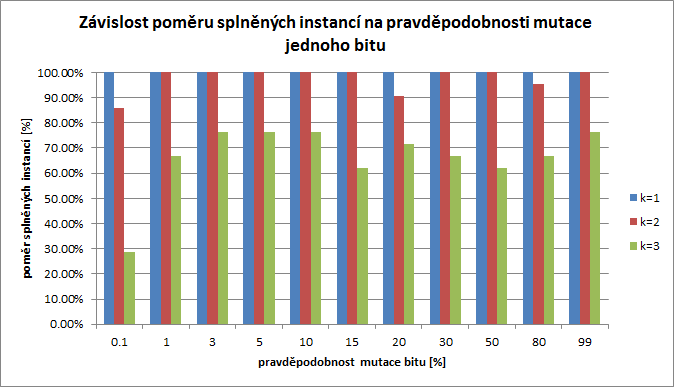
\includegraphics[scale=0.9]{obr/mut-sat.png}
\end{figure}
\newpage
\FloatBarrier

\subsection{Meření závislostí pravděpodobnosti a typu křížení}

V rámci měření závislosti relativní chyby na pravděpodobnosti křížení byla porovnáván i vliv jednotlivých typů implementovaných křížení na kvalitě dosažených řešení.

Pravděpodobnost křížení určuje, zda v rámci aktuální generace dochází k vzniku nové genetické informace výběrem zdatných jedinců (rodičů) z generace předchozí jejich rekombinací. V případě, kdy je vliv křížení utlumen snížením pravděpodobnosti, zůstává za vznik nové genetické informace zodpovědný pouze operátor mutace, což může prodloužit celkovou dobu konvergence algoritmu k opt. řešení.

Všechny implementované typy křížení řešily instance s podobnými relativními chybami a nebyl sledován jejich vliv na výsledků řešení. 

Dále je z naměřených výsledků patrné, že všechna nastavení pravděpodobnosti křížení nižší než 99\% generují poměrně značné rel. chyby. Dalším zajímavým úkazem je, že na rozdíl od pst. mutace, pokles pravděpodobnosti křížení významně negativně ovlivňuje i splnitelnost řešení vracených heuristikou.

\begin{figure}[ht]
\centering
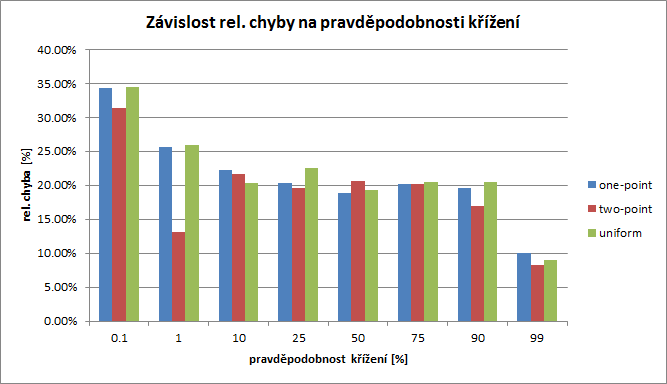
\includegraphics[scale=0.9]{obr/cross-err.png}
\end{figure}


\begin{figure}[ht]
\centering
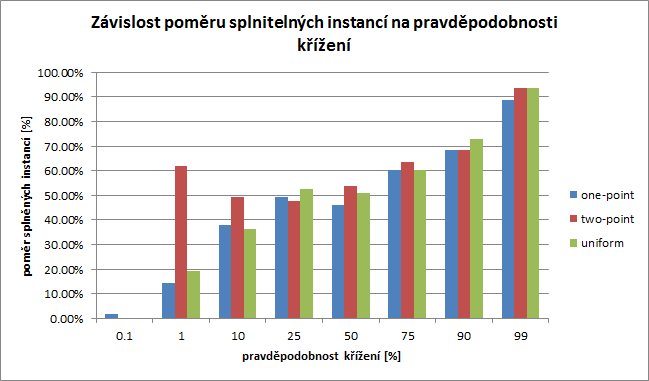
\includegraphics[scale=0.9]{obr/cross-sat.png}
\end{figure}

\newpage
\FloatBarrier

\subsection{Meěení vlivu nastavení škálovací funkce 1}

Jak již bylo uvedeno v předchozí podkapitole, k zvýšení selekčního tlaku dochází u první metody pro hodnoty koeficientu $c_s < 0$ Naopak snížení sel. tlaku a tedy nadržování slabším jedincům dochází u hodnot koeficientu $c_s > 0$.

Z grafu je možné vypozorovat, že k mírnému zvýšení kvality řešení je dosaženo při snížením selekčního tlaku nastavením hodnoty koeficientu $k=0,7$. Toto zajistí menší důraz na výběr těch nejlepších jedinců v rámcí výběru instancí pro operaci křížení a zabrání tak k případné degeneraci populace.
/

\begin{figure}[ht]
\centering
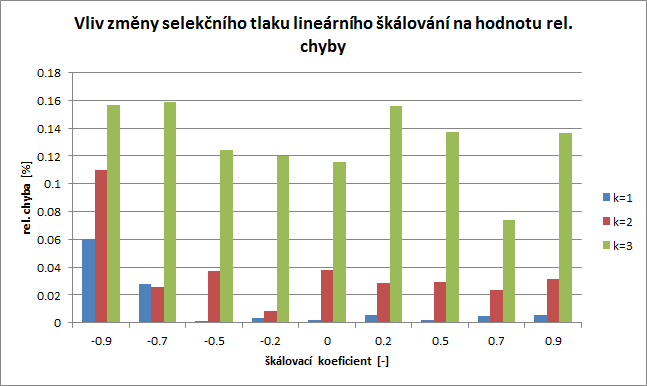
\includegraphics[scale=0.9]{obr/linscale-err.png}
\end{figure}

\begin{figure}[ht]
\centering
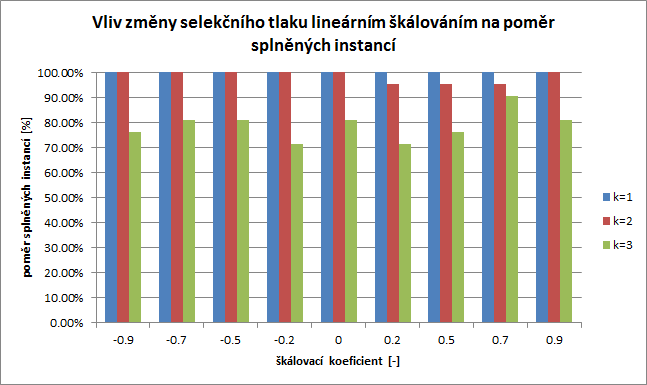
\includegraphics[scale=0.9]{obr/linscale-sat.png}
\end{figure}
\newpage
\FloatBarrier

\subsection{Měření vlivu nastavení škálovací funkce 2}

Snížení selekčního tlaku se ukázalo jako výhodné i v případě druhé metody. Zde se jako doporučené nastavení hodnoty škálovacího koeficientu jeví hodnoty $c_s=0,7$, tedy nastavení nové hodnoty zdatnosti nejlepšího jedince na přibližně 0,7 násobek původní průměrné hodnoty zdatnosti celé populace.

\begin{figure}[ht]
\centering
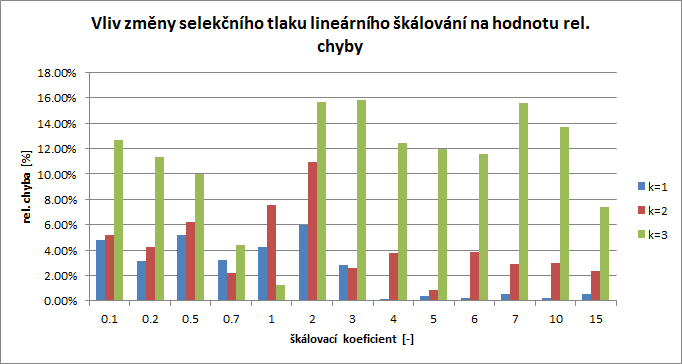
\includegraphics[scale=0.9]{obr/linavgscale-err.png}
\end{figure}

\FloatBarrier
\newpage

\subsection{Měření vlivu nastavení penalizací}

Jak již bylo zmíněno dříve, jedním z cílů tohoto experimentu, bylo najít takové parametry, se kterými dokáže heuristika řešit i ty nejobtížnější instance. Žádný z dosud testovaných parametrů neměl bohužel na špatnou kvalitu řešení nejtěžších instancí vliv.

Toto se podařilo změnit až změnou volby penalizační funkce, kde byla nahrazena nevhodná penalizace (založená na vynásobení fitness hodnoty nesplněné instance poměrem splněných klauzulí ku počtu všech klauzulí) za penalizaci aditivní zohledňující váhy literálů v nesplněných klauzulích. Teto metoda penalizace je pak u velmi špatných konfigurací mnohem přísnější než metoda původní.

Z grafu je patrné, že nejlepších výsledků dosahuje heuristika při použití aditivní penalizace znásobené váhou $c_p = 4$.

\begin{figure}[ht]
\centering
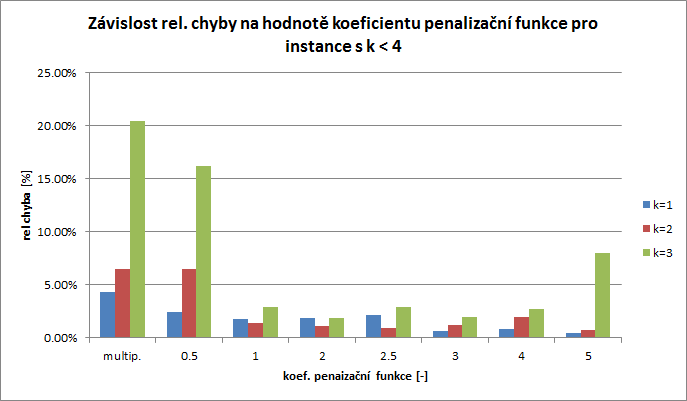
\includegraphics[scale=0.9]{obr/pen-err-min.png}
\end{figure}

\begin{figure}[ht]
\centering
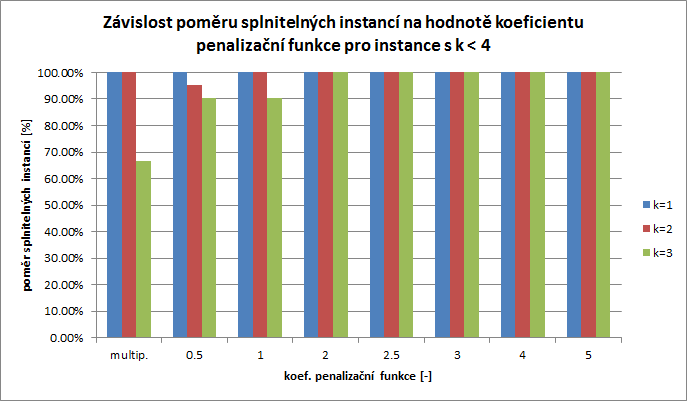
\includegraphics[scale=0.9]{obr/pen-sat-min.png}
\end{figure}

\begin{figure}[ht]
\centering
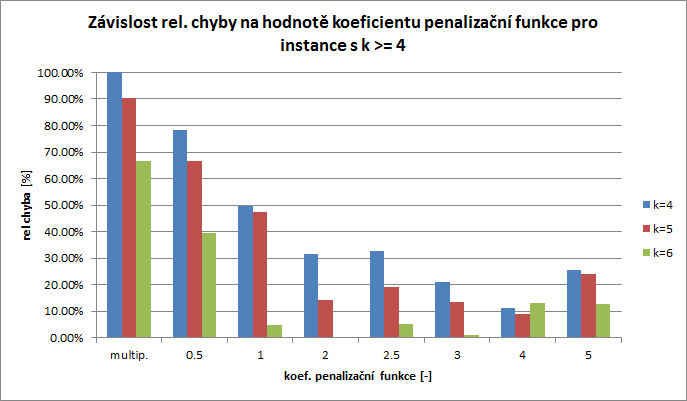
\includegraphics[scale=0.9]{obr/pen-err-max.png}
\end{figure}

\begin{figure}[ht]
\centering
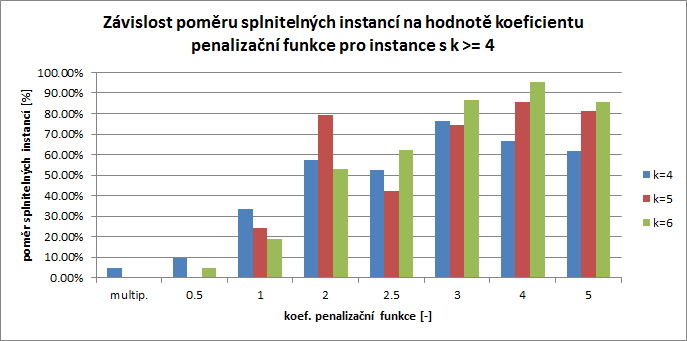
\includegraphics[scale=0.9]{obr/pen-sat-max.png}
\end{figure}
\FloatBarrier
\newpage

\section{Poznámky k implementaci}

Řešení bylo implementováno jako rozšíření výukové knihovny, která je součástí studijních materiálů kurzu \uv{Artificial Intelligence: A Modern Approach} univerzity Berkeley. Tato knihovna byla rozšířena o podporu optimalizačních problémů, pro které byly implementován problém batohu a problém splnitelnosti booleovské formule. Implementované řešení je jednoduše rozšiřitelné o další typy problémů nebo heuristik, které tyto problémy řeší. Jazykem implementace je Common LISP.


\section{Závěr}
\begin{itemize}
\item Překvapivým závěrem bylo zjištění nezávislosti kvality podávaných výsledků heuristikou na typu křížení.
\item Úspěchem se ukázala být volba aditivní penalizační funkce znevýhodňující nesplnitelné instance odečtením maximálních vah literálů nesplnitelných klauzulí. Při aplikaci této funkce je dosahováno podstatně lepších výsledků (zejména pro ty těžší problémy) než je tomu u multiplikativní penalizace založené na poměru nesplněných klauzulí.
\item Jako velkou nevýhodou při porovnání výsledků heuristiky se projevilo zahrnutí nesplnitelných instancí (tj. instancí, které nevedly k výsledku) do výpočtu relativní chyby.
\item Výsledky (zejména experimentu zobrazujícího vliv velikosti populace) potvrzují závěry Selmana, kdy jsou jako nejobtížnější instance označovány ty, které mají poměr počtu klauzulí k počtu proměnných blízký hodnotě 4,5. Tato skutečnost se v rámci experimentů opravdu potvrdila. Kvalitativně nejhorších výsledků bylo dosahováno pro instance s $k=4$ a $k=5$.
\item Zajímavým rozšířením heuristiky, dle mého názoru spočívá v implementaci dalších selekčních metod jako je např. univerzální stochastické vzorkování nebo turnajový výběr a jejich vzájemné porovnání.

\end{itemize}

\section{Literatura}
\begin{itemize}
\item Scaling in Genetic Algorithms - Sushil J. Louis - \url{http://www.cse.unr.edu/~sushil/class/gas/notes/scaling/index.html}
\item Stochastic Search And Phase Transitions:AI Meets Physics. Bart Selman, AT\&T Bell Laboratories, Murray Hill, N.J. USA
\end{itemize}


\renewcommand{\refname}{Literatura}
\bibliographystyle{ieeetr}
{
 \bibliography{refs}
}


\end{document}
